\documentclass[12pt]{extarticle}
%Some packages I commonly use.
\usepackage[portuguese]{babel}
\usepackage{graphicx}
\usepackage{framed}
\usepackage[normalem]{ulem}
\usepackage{amsmath}
\usepackage{amsthm}
\usepackage{amssymb}
\usepackage{amsfonts}
\usepackage{enumerate}
\usepackage[utf8]{inputenc}
\usepackage{float}
\usepackage{gensymb}
\usepackage[top=1 in,bottom=1in, left=1 in, right=1 in]{geometry}
\usepackage{multirow}
\usepackage{caption}
\usepackage{subcaption}
\usepackage[utf8]{inputenc}

%A bunch of definitions that make my life easier
\newcommand{\matlab}{{\sc Matlab} }
\newcommand{\cvec}[1]{{\mathbf #1}}
\newcommand{\rvec}[1]{\vec{\mathbf #1}}
\newcommand{\ihat}{\hat{\textbf{\i}}}
\newcommand{\jhat}{\hat{\textbf{\j}}}
\newcommand{\khat}{\hat{\textbf{k}}}
\newcommand{\minor}{{\rm minor}}
\newcommand{\trace}{{\rm trace}}
\newcommand{\spn}{{\rm Span}}
\newcommand{\rem}{{\rm rem}}
\newcommand{\ran}{{\rm range}}
\newcommand{\range}{{\rm range}}
\newcommand{\mdiv}{{\rm div}}
\newcommand{\proj}{{\rm proj}}
\newcommand{\R}{\mathbb{R}}
\newcommand{\N}{\mathbb{N}}
\newcommand{\Q}{\mathbb{Q}}
\newcommand{\Z}{\mathbb{Z}}
\newcommand{\<}{\langle}
\renewcommand{\>}{\rangle}
\renewcommand{\emptyset}{\varnothing}
\newcommand{\attn}[1]{\textbf{#1}}
\theoremstyle{definition}
\newtheorem{theorem}{Theorem}
\newtheorem{corollary}{Corollary}
\newtheorem*{definition}{Definition}
\newtheorem*{example}{Example}
\newtheorem*{note}{Note}
\newtheorem{exercise}{Exercise}
\newcommand{\bproof}{\bigskip {\bf Proof. }}
\newcommand{\eproof}{\hfill\qedsymbol}
\newcommand{\Disp}{\displaystyle}
\newcommand{\qe}{\hfill\(\bigtriangledown\)}
\setlength{\columnseprule}{1 pt}
\usepackage[utf8]{inputenc}

\title{Aula 14 - Geradores, Receptores e Capacitores}
\author{Felipe Salvador}
\date{Atualizado em \today}

\begin{document}

\maketitle

\section{Introdução}

Nessa aula, iremos ver os outros tipos de equipamentos elétricos que podemos colocar num circuito e como eles influenciam o funcionamento de um circuito. Faremos as análises de como se encontra os resultados necessários para a solução.

\section{Geradores Elétricos}
Os geradores são uma classe de equipamentos elétricos que fornece energia ao sistema. Sem eles, o funcionamento do circuito não aconteceria. Num circuito, o gerador é dado pelo símbolo:

\begin{figure}[H]
    \centering
    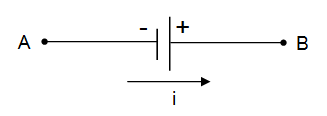
\includegraphics[width=0.6\textwidth]{a1.PNG}
    \caption{Diagrama de um gerador num circuito}
    \label{fig:gerador}
\end{figure}

Importante notar que \textbf{a corrente sempre sai do pólo positivo.} A relação de um gerador é dada por:
\begin{equation}
    U= \varepsilon - R\,i
\end{equation}
\noindent que $U$ é a d.d.p., $R$ é a resistência do circuito, $i$ é a corrente que passa no circuito e $\varepsilon$ é a chamada \textbf{força eletromotriz}. A unidade de $\varepsilon$ é Volt (V). \textbf{Sempre que um exercício der um valor em volt de um gerador, o exercício está dando o valor da Força Eletromotriz do gerador ($\varepsilon$)}.

Num gerador, a força eletromotriz ($\varepsilon$) é definida e constante, ou seja, a d.d.p. vai depender da resistência e corrente que passa no circuito. Porém, existe uma corrente máxima que o gerador consegue fornecer, para valores maiores que ela, o gerador queima. Essa corrente é chamada \textbf{corrente de curto circuito} ($i_{cc}$) e acontece quando a d.d.p. produzida é 0:
\begin{equation}
    0= U = \varepsilon - R\,i_{cc} \implies \boxed{ i_{cc} = \frac{\varepsilon}{R}}
\end{equation}

A potência de um gerador é dada por: $P = U\,i$, em que vimos que $U = \varepsilon - R\,i$. Substituindo essa relação na fórmula da potência:
\begin{equation}
    P = (\varepsilon - R\,i)\,i \implies P = \varepsilon\,i - R\,i^2
\end{equation}
\noindent que $\varepsilon\,i = P_t$ é a potência total que um gerador pode produzir e $R\,i^2 = P_d$ é a potência dissipada/perdida pelo próprio gerador. Logo:
\begin{equation}
    P = P_t - P_d \implies P = \text{Potência útil do gerador.}
\end{equation}

Com isso, podemos calcular o rendimento ($\eta$) desse gerador:
\begin{equation}
    \eta = \frac{P}{P_t}
\end{equation}

Essa quantidade me diz o quanto bom o gerador é na produção de energia. Se o rendimento é próximo de 1, isso significa que ele consegue entregar quase toda a energia que ele consegue fornecer, ou seja, muito pouca energia é perdida por dissipação.

\subsection{Associação de geradores}
\subsubsection{Geradores em série}
Quando colocamos geradores em série, \textbf{a corrente que passa por eles é a mesma.}

Como a d.d.p. fornecida por um gerador é: $U_1 = \varepsilon_1 - R_1\,i$, para os geradores em série, a d.d.p. total gerada é a soma da d.d.p gerada por cada gerador:
\begin{equation}
    \begin{split}
        U &= U_1 + U_2 + U_3 + U_4\\
        U &= \varepsilon_1 - R_1\,i + \varepsilon_2 - R_2\,i + \varepsilon_3 - R_3\,i + \varepsilon_4 - R_4\,i\\
        U &= (\varepsilon_1 + \varepsilon_2 + \varepsilon_3 + \varepsilon_4) - (R_1 + R_2 + R_3 + R_4)\,i
    \end{split}
\end{equation}

Como a d.d.p. gerada um gerador é: $U = \varepsilon - R\,i$, a equação anterior nos diz que a associação em série de geradores pode ser substituída por um gerador equivalente com as forças eletromotriz e resistência igual à:
\begin{equation}
    \boxed{\begin{split}
        \varepsilon_{eq} &= \varepsilon_1 + \varepsilon_2 + \varepsilon_3 + \varepsilon_4\\
        R_{eq} &= R_1+R_2+R_3+R_4
    \end{split}}
\end{equation}
\begin{figure}[H]
    \centering
    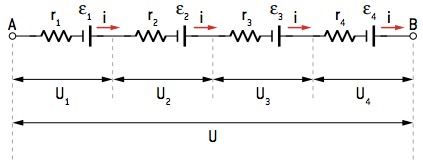
\includegraphics[width=0.5\textwidth]{20200505-associacao-geradores2.png}
    \caption{Diagrama de geradores em série}
    \label{fig:associacao_em_serie}
\end{figure}

\textbf{De forma geral, quando temos geradores em série, eles podem ser substituídos por um gerador equivalente cuja força eletromotriz é a soma das forças dos geradores e a resistência é a soma das resistências.}

\subsubsection{Geradores em paralelo}

Quando colocamos geradores em paralelo, \textbf{a d.d.p. produzida por cada gerador é a mesma}. Nós só vamos analisar o caso em que cada gerador possui a mesma força eletromotriz e resistência interna.

\begin{figure}[H]
    \centering
    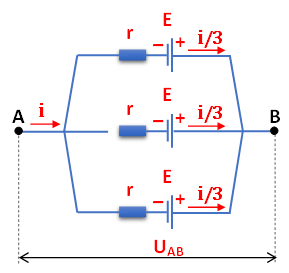
\includegraphics[width=0.5\textwidth]{gerador_paralelo.png}
    \caption{Diagrama de geradores em paralelo}
    \label{fig:associacao_em_paralelo}
\end{figure}

Para cada gerador:
\begin{equation}
    U = \varepsilon - R\,\frac{i}{3}
\end{equation}

 Para um gerador equivalente aos geradores associados em paralelo:
\begin{equation}
    U = \varepsilon_{eq} - R_{eq}\,i
\end{equation}

Comparando as duas últimas equações:
\begin{equation}
    \boxed{\begin{split}
        \varepsilon_{eq} &= \varepsilon\\
        R_{eq} &= \frac{R}{3}
    \end{split}}
\end{equation}

Esse resultado pode ser generalizado. Para um número 'n' de geradores em paralelo:
\begin{equation}
    \boxed{\begin{split}
        \varepsilon_{eq} &= \varepsilon\\
        R_{eq} &= \frac{R}{n}
    \end{split}}
\end{equation}

\section{Receptor Elétrico}

São equipamentos elétricos que transformam a energia elétrica em alguma outra energia, diferente da energia térmica. Um exemplo de receptor é celular, computador, televisão e assim por diante. No circuito, ele tem um diagrama muito parecido com o do gerador elétrico.

\begin{figure}[H]
    \centering
    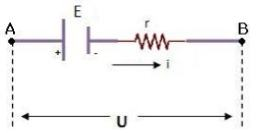
\includegraphics[width=0.5\textwidth]{receptor-eletrico.jpg}
    \caption{Diagrama de um receptor elétrico}
    \label{fig:receptor}
\end{figure}

\textbf{Importante ressaltar que, para um receptor, a corrente (i) sai do polo negativo, diferentemente de um gerador, que a corrente sai do polo positivo.}

A equação para um receptor é dada por:
\begin{equation}
    U = \varepsilon' + R\,i
\end{equation}
\noindent em que $U$ é a d.d.p que o receptor está, $\varepsilon'$ é a \textbf{força contra-eletromotriz}, $R$ é a resistência interna e $i$ é a corrente que passa por ele. A unidade da força contra-eletromotriz é Volt (V). \textbf{Sempre que um exercício der um valor em volt de um receptor, o exercício está dando o valor da Força Contra-eletromotriz do gerador ($\varepsilon$)}.

As relações de associação de receptores são as mesmas do caso dos geradores.
\subsection{Como diferenciar um gerador de um receptor}

Normalmente, num circuito, não se tem informação sobre qual é a direção que a corrente está fazendo. Logo, se tivermos um gerador e um receptor no circuito, a princípio não conseguimos saber quem é o gerador e quem é o receptor, como no caso abaixo:
\begin{figure}[H]
    \centering
    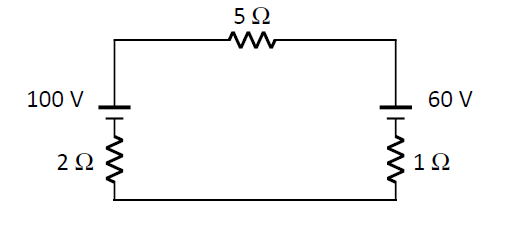
\includegraphics[width=0.5\textwidth]{ex_1.png}
    \label{fig:ex_1}
\end{figure}

Bem primeiramente, os dois são geradores, receptores ou um é gerador e o outro é receptor? \textbf{Um é receptor e o outro é gerador, porque os polos positivos estão no mesmo lado do circuito, ou seja, a linha que sai de um polo positivo chega ao polo positivo do outro.}

Bem, como um é gerador e o outro é receptor, quem é quem? \textbf{O gerador sempre é aquele que possui a força eletromotriz maior. O outro, por consequência, é o receptor.} Como no circuito, há 2 informações sobre a força eletromotriz (100 e 60 V), então \textbf{o gerador é o equipamento com a força e eletromotriz de 100 V e o receptor é o equipamento com a força contra-eletromotriz de 60V}.

\section{Capacitores}
São equipamentos elétricos que acumulam carga para o uso posterior, como estabilizadores de tensão, por exemplo. Enfim, os capacitores são dados no circuito pega seguinte figura:
\begin{figure}[H]
    \centering
    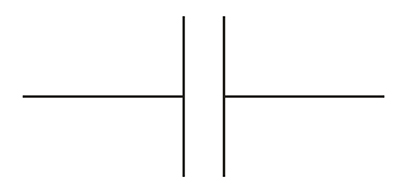
\includegraphics[width=0.4\textwidth]{capacitor.png}
    \caption{Diagrama de um capacitor num circuito}
    \label{fig:capacitor}
\end{figure}

Em geral, os capacitores que iremos tratar são os capacitores de placas paralelas. Nas placas do capacitor, ele acumula cargas elétrica, conforme a figura abaixo:
\begin{figure}[H]
    \centering
    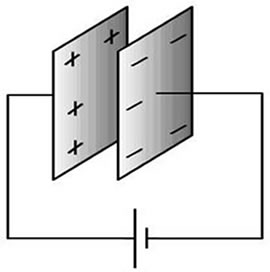
\includegraphics[width=0.5\textwidth]{capacitor_placas_paralelas.jpg}
    \caption{Como as cargas se acumulam no capacitor}
    \label{fig:placas_paralelas}
\end{figure}

A equação que descreve um capacitor é dada por:
\begin{equation}
    Q=C\,U
\end{equation}
\noindent em que $Q$ é a carga total acumulada por um capacitor, $U$ é a d.d.p. em que o capacitor está e $C$ é chamado de \textbf{capacitância}.

A capacitância me diz o quanto de cargas elétrica um capacitor consegue comportar. Quanto mais cargas, maior será a capacitância. A unidade da capacitância é dada em \textbf{Farad (F)}.

A energia elétrica que um capacitor comporta é dada por:
\begin{equation}
    E = \frac{Q\,U}{2} = \frac{Q^2}{2C} = \frac{C\,U^2}{2}
\end{equation}

\subsection{Associação de Capacitores}
Em geral, a associação de capacitores funciona de uma forma similar à associação de resistores.

Para a associação de resistores:
\begin{equation}
    \begin{split}
        R_{eq} &= R_1 + R_2 + R_3 +\dots\, \,\text{(Resistores em série)}\\
        \frac{1}{R_{eq}} &= \frac{1}{R_1} + \frac{1}{R_2} + \frac{1}{R_3} + \dots\,\, \text{(Resistores em paralelo)}
    \end{split}
\end{equation}

Já para os capacitores:
\begin{equation}
    \boxed{\begin{split}
        \frac{1}{C_{eq}} &= \frac{1}{C_1} + \frac{1}{C_2} + \frac{1}{C_3} + \dots\,\, \text{(Capacitores em série)}\\
        C_{eq} &= C_1 + C_2 + C_3 +\dots\, \,\text{(Capacitores em paralelo)}
    \end{split}}
\end{equation}
\end{document}
